\documentclass{amsart}          

% PACKAGES ~~~~~~~~~~~~~~~~~~~~

\usepackage{amsfonts}
\usepackage{amssymb}  
\usepackage{amsthm} 
\usepackage{amsmath} 
\usepackage{caption}
\usepackage[inline]{enumitem}
    \setlist{itemsep=0em, topsep=0em, parsep=0em}
    \setlist[enumerate]{label=(\alph*)}
\usepackage{doi}
\usepackage{etoolbox}
\usepackage{stmaryrd} 
\usepackage[dvipsnames]{xcolor}
    \definecolor{editcolour}{rgb}{0.7,0.1,0}
    \definecolor{hrefcolour}{rgb}{0,0,0.7}
\usepackage[]{hyperref}
    \hypersetup{colorlinks,linkcolor={hrefcolour},citecolor={hrefcolour},urlcolor={hrefcolour}}
\usepackage{graphicx}
    \graphicspath{ {img/} }
\usepackage{mathtools}
\usepackage[numbers]{natbib}
\usepackage{subcaption}
\usepackage{subfiles}
\usepackage{tikz}
    \usetikzlibrary{matrix,arrows,shapes,decorations.markings,decorations.pathreplacing}
\usepackage{todonotes}
\usepackage{url}

% NEW COMMANDS ~~~~~~~~~~~~~~~~~~

% mathbb
%\newcommand{\RR}{\mathbb{R}}
%\newcommand{\ZZ}{\mathbb{Z}}
%\newcommand{\NN}{\mathbb{N}}
%\newcommand{\QQ}{\mathbb{Q}}
%\newcommand{\CC}{\mathbb{C}}
%\newcommand{\FF}{\mathbb{D}}

% symbols
\renewcommand{\epsilon}{\varepsilon}
\newcommand{\op}{^{ \text{op} }}
\newcommand{\ob}{_{ \text{ob} }}
\newcommand{\arr}{_{ \text{arr} }}
\newcommand{\lin}{_{\t{lin}}}
\newcommand{\iso}{\cong}
\renewcommand{\equiv}{\simeq}

% categories
\newcommand{\A}{\cat{A}}
\newcommand{\B}{\cat{B}}
\newcommand{\C}{\cat{C}}
\newcommand{\D}{\cat{D}}
\renewcommand{\P}{\cat{P}}
\newcommand{\X}{\cat{X}}
\newcommand{\Y}{\cat{Y}}
\newcommand{\Z}{\cat{Z}}
\renewcommand{\AA}{\bicat{A}}
\newcommand{\BB}{\bicat{B}}
\newcommand{\CC}{\bicat{C}}
\newcommand{\PP}{\bicat{P}}
\newcommand{\XX}{\bicat{X}}
\newcommand{\YY}{\bicat{Y}}
\newcommand{\ZZ}{\bicat{Z}}
\newcommand{\AAA}{\dblcat{A}}
\newcommand{\BBB}{\dblcat{B}}
\newcommand{\CCC}{\dblcat{C}}
\newcommand{\PPP}{\dblcat{P}}
\newcommand{\XXX}{\dblcat{X}}
\newcommand{\YYY}{\dblcat{Y}}
\newcommand{\ZZZ}{\dblcat{Z}}

\newcommand{\Set}{\cat{Set}}
\newcommand{\Graph}{\cat{Graph}}
\newcommand{\RGraph}{\cat{RGraph}}
\newcommand{\Top}{\cat{Top}}
\newcommand{\Cat}{\cat{Cat}}
\newcommand{\Bicat}{\cat{Bicat}}
\newcommand{\DblCat}{\cat{DblCat}}
\newcommand{\Topos}{\cat{Topos}}
\newcommand{\Gram}{\cat{Gram}}
\newcommand{\StrCspGram}{\cat{StrCspGram}}
\newcommand{\Span}[1]{\cat{Span}(#1)}
\newcommand{\Csp}[1]{\cat{Csp}(#1)}
\newcommand{\StrCsp}{\cat{StrCsp}}
\newcommand{\SStrCsp}{\bicat{StrCsp}}
\newcommand{\SSStrCsp}{\mathbb{S}\cat{stCsp}}
\newcommand{\Rewrite}{\cat{Rewrite}}
\newcommand{\RRewrite}{\bicat{Rewrite}}
\newcommand{\RRRewrite}{\mathbb{R}\mathbf{ewrite}}
\newcommand{\MonRewrite}{\cat{MonRewrite}}
\newcommand{\MMonRewrite}{\bicat{MonRewrite}}
\newcommand{\MMMonRewrite}{\dblcat{M}\bicat{onRewrite}}

% functors
\newcommand{\core}{\mathbf{core}}
\newcommand{\Lang}{\mathcal{L}}

% text formatting
\newcommand{\defn}[1]{\textbf{#1}}
\newcommand{\cat}[1]{\mathrm{#1}}
\newcommand{\bicat}[1]{\mathbf{#1}}
\newcommand{\dblcat}[1]{\mathbb{#1}}
\newcommand{\type}[1]{\mathtt{#1}}
\renewcommand{\t}[1]{\text{#1}}
\newcommand{\edit}[1]{\textcolor{editcolour}{(#1)}}

% arrows
\newcommand{\from}{\colon}
\newcommand{\rel}{\nrightarrow}
\newcommand{\xto}[1]{\xrightarrow{#1}}
\newcommand{\xgets}[1]{\xleftarrow{#1}}
\newcommand{\tospan}{\xrightarrow{\mathit{sp}}}
\newcommand{\spn}[3]{#1 + #3 \to #2}
\newcommand{\csp}[3]{#2 \to #1 \times #3}
\newcommand{\tocospan}{\xrightarrow{\mathit{csp}}}
\newcommand{\diagram}[1]{\raisebox{-0.5\height}{\includegraphics{#1}}}


% MATH OPERATORS ~~~~~~~~~~~~~~~~~~

\DeclareMathOperator{\Hom}{Hom}
\DeclareMathOperator{\id}{id}
\DeclareMathOperator{\im}{im}
\DeclareMathOperator{\Aut}{Aut}
\DeclareMathOperator{\Bij}{Bij}
\DeclareMathOperator{\Sub}{Sub}
\DeclareMathOperator{\colim}{colim}

% ENVIRONMENTS & COUNTERS ~~~~~~~~~~~

\newtheorem{theorem}{Theorem}[section]
\newtheorem{lemma}[theorem]{Lemma}
\newtheorem{proposition}[theorem]{Proposition}
\newtheorem{corollary}[theorem]{Corollary}

\theoremstyle{remark}
\newtheorem{remark}[theorem]{Remark}
\newtheorem{notation}[theorem]{Notation}

\theoremstyle{definition}
\newtheorem{example}[theorem]{Example} 
\newtheorem{definition}[theorem]{Definition}

\setcounter{tocdepth}{1} % Sets depth for table of contents. 

% TIKZ TYPES ~~~~~~~~~~~~~~~~~~~~~

% arrow head in middle of edge
\tikzset{->-/.style={decoration={%
      markings,
      mark=at position .5 with {\arrow{>}}},postaction={decorate}}
}

% arrow head user-positioned
\tikzset{->-pos/.style={decoration={%
      markings,
      mark=at position #1 with {\arrow{>}}},postaction={decorate}}
}

% arrow head in middle of edge
\tikzset{-|->/.style={decoration={%
      markings,
      mark=at position .5 with {\arrow{|}},mark=at position 1 with {\arrow{>}}},postaction={decorate}}
}

% INLINE DIAGRAMS ~~~~~~~~~~~~~~~

% walking reflexive graph
\newcommand{\rgraph}[2]{%
  $\begin{tikzpicture}
    \node (a) at (0,0) {$ #1 $};
    \node (b) at (1,0) {$ #2 $};
    \draw [->] (a.30) to (b.150);
    \draw [->] (a.-30) to (b.-150);
    \draw [->] (b) to (a);
  \end{tikzpicture}$
}

% walking graph
\newcommand{\graph}[2]{%
  $\begin{tikzpicture}
    \node (a) at (0,0) {$ #1 $};
    \node (b) at (1,0) {$ #2 $};
    \draw [->] (a.15) to (b.165);
    \draw [->] (a.-15) to (b.-165);
  \end{tikzpicture}$
}

% open tipped arrow
\newcommand{\opento}[2]{%
  \begin{tikzpicture}
  \node (a) at (0,0) {$ #1 $};
  \node (b) at (1,0) {$ #2 $};
  \draw [->, open triangle 60] (a) to (b);
  \end{tikzpicture}
}

% inline horizontal arrow
\newcommand{\horarrow}[2]{%
  \begin{tikzpicture}
    \node (a) at (0,0) {$ #1 $};
    \node (b) at (1,0) {$ #2 $};
    \draw [-|->] (a) to (b);
  \end{tikzpicture}
}

% adjunction
\newcommand{\adjunction}[4]{%
  \begin{tikzpicture}
    \node (1) at (0,0) {\( #1 \)};
    \node (2) at (2,0) {\( #4 \)};
    \node (3) at (1,0) {\scriptsize{\( \perp \)}};
    \draw [->] (2.135) to node [above] {\scriptsize{ $ #2 $ }} (1.45);
    \draw [->] (1.-45) to node [below] {\scriptsize{ $ #3 $ }} (2.-135);
  \end{tikzpicture}
%
}

\author{Daniel Cicala}
\title{Rewriting structured cospans}

% ~~~~~~~~~~~~~~~~~~~~~~~~~~~~~~~~~~~~~~~~
% 
% ~~~~~~~~~~~ end preamble ~~~~~~~~~~~~~~~
% 
% ~~~~~~~~~~~~~~~~~~~~~~~~~~~~~~~~~~~~~~~~

\begin{document}

\maketitle{}


% ~~~~~~~~~~~~~~~~~~~~~~~~~~~~~~~~~~~~~~~~
% ~~~~~~~~~~~~~~~~~~~~~~~~~~~~~~~~~~~~~~~~
% ~~~~~~~~~~~~~~~~~~~~~~~~~~~~~~~~~~~~~~~~
% ~~~~~~~~~~~~~~~~~~~~~~~~~~~~~~~~~~~~~~~~

\section{Introduction}
\label{sec:intro}

\section{Structured cospans}
\label{sec:cat-of-strcsp}

Structured cospans were introduced to model compositional systems. In
fact, they were the second approach to model compositional systems
using cospans.  Fong invented \emph{decorated cospans}
%
\todo{cite decorated cospans}
%
, the first approach.  Structure cospans are
introduced here as well as by Baez and Courser.
%
\todo{cite baez-courser strcsp}
%
The latter has work two aims: maximize the
generality of the structured cospan construction using double
categories and also to compare decorated and structured cospans. Our
present interests are focused on introducing rewriting on structured
cospans, hence we will make a number of restrictions that Baez and
Courser do not.  These restriction are harmless, however, as most
cases of interest fall within the our parameters.

In this section, we will make explicit two perspectives on structured
cospans, both through the language of category theory.  The first is
looking at structured cospans as an object with morphisms between
them. The second is as a morphism between ``interfaces''.  It is the
latter perspective that encodes the compositional structure.  

% define a category of open networks

For good, we fix a geometric morphism $ L \dashv R \from \X \to \A
$. This is an adjunction
%
\[
  \begin{tikzpicture}
    \node (1) at (0,0) {\( \X \)};
    \node (2) at (2,0) {\( \A \)};
    \node (3) at (1,0) {\scriptsize{\( \perp \)}};
    \draw [<-] (1.45) to node [above] {\scriptsize{\(  L \)}} (2.135);
    \draw [<-] (2.-135) to node [below] {\scriptsize{ $ R $ } } (1.-45);
  \end{tikzpicture}
\]
%
between (elementary) topoi with $ L $ left exact.

Our motivations being the modeling of open systems, beginning
the story by fixing a geometric morphism might signal the abstract
nature of this work and obfuscate the connection between structured
cospans and open systems. So that we do not drift too far from our
concrete motivations, we will draw analogies between our construction
and open systems throughout.  

Here is the first such analogy. One should view the topos $ \A $ as
consisting of closed systems and their morphisms. By a \emph{closed
  system}, we mean a system that cannot interact with the outside
world. The topos $ \X $ should be thought to contain possible
interfaces for the closed systems. Equipping a closed system with an
interface provides an avenue for the system to now interact with
compatible elements of the outside world. The interface dictates
compatibility as we explore below.  Such a system is no longer closed,
and so we call it an \emph{open system}. The left adjoint $ L $ sends
these interfaces into $ \X $ so that they might interact with the
closed systems. The right adjoint $ R $ can be though of as returning
a closed system's largest possible interface. A word of caution: this
is an informal analogy and should only be used to gain an intuition
for the nature of structured cospans. Now, let us turn to the first of
two perspectives on structured cospans.

\subsection{Structure cospans as objects}
\label{sec:strcsp-as-object}

% introduce the section

In this section, we define a structured cospan and the appropriate
notion of morphism. The main result of the section is that the
corresponding category is a topos in a functorial way.

\begin{definition}\label{df:strcsp}

  A \defn{ structured cospan } is a cospan of the form
  $ La \to x \gets Lb $.
  
\end{definition}

To typeset cospans inline, we will writing them as $
\csp{x}{y}{z} $ and spans as $ \spn{x}{y}{z} $. Because all of the
categories in this paper will have products and coproducts, this
notation is sensible.  

There is no novelty in a simple cospan, but we present this as a new
definition to place ourselves into the context of systems
modelling. Also, the reason for restricting ourselves to a geometric
morphism at this point is elusive. Especially so because the other
introducory work on structured cospans by Baez and Courser did not ask
for this. Let us say that this requirement arises from practical and aesthetic
considerations. For one, a nicer theory develops, but also it is a
sufficiently strong condition to introduce rewriting of structured cospans.

Returning briefly to the systems analogy, a structured cospan consists
of a closed system $ x $ with an interface identified by the arrows
from $ La $ and $ Lb $. Ignoring questions of causality, it is safe to
consider $ La $ as the input to $ x $ and $ Lb $ as the output. The
sum total of the closed system $ x $ equipped with interface
$ La + Lb $ is our open system. As expected, a morphism of open system
ought to respect these components.

\begin{definition} \label{df:morph-of-strcsp}

  A morphism from one structured cospan
  %
  \(
  \csp{La}{x}{Lb}
  \)
  %
  to another
  %
  \(
    \csp{Lc}{y}{Ld}
  \)
  % 
  is a triple of arrows $ ( f,g,h ) $ that fit into the commuting
  diagram
  \[
    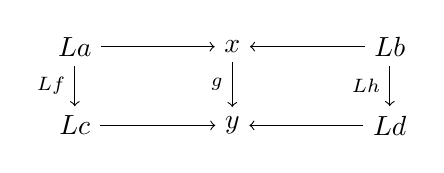
\begin{tikzpicture}
      \node (1) at (-2,1) {\( La \)};
      \node (2) at (0,1) {\( x \)};
      \node (3) at (2,1) {\( Lb \)};
      \node (4) at (-2,0) {\( Lc \)};
      \node (5) at (0,0) {\( y \)};
      \node (6) at (2,0) {\( Ld \)};
      \draw [->] (1) to node [above] {\scriptsize{\(  \)}} (2);
      \draw [->] (3) to node [above] {\scriptsize{\(  \)}} (2);
      \draw [->] (4) to node [below] {\scriptsize{\(  \)}} (5);
      \draw [->] (6) to node [below] {\scriptsize{\(  \)}} (5);
      \draw [->] (1) to node [left] {\scriptsize{\( Lf \)}} (4);
      \draw [->] (2) to node [left] {\scriptsize{\( g \)}} (5);
      \draw [->] (3) to node [left] {\scriptsize{\( Lh \)}} (6);
    \end{tikzpicture}
  \]
\end{definition}

It is a simple exercise to show that structured cospans and their
morphisms form a category.  Denote this category by $ \StrCsp\ob
$. This subscript reminds us that structured cospans are objects in
this category. In fact, we willl refer to the objects of this category
as a \defn{structured cospan category}. While this category does
depend on additional data, minimally $ L $, we suppress this from the
notation and rely on context. When wanting to be explicit, we will
write $ \StrCsp\ob ( L ) $.

% examples of open networks

\begin{example}[Open graphs] \label{ex:open-graphs}

  The field of network theory is intimately tied with graph theory
  \cite{networks}. A natural example of a structured is an \emph{open
    graph}. While this notion is not new,
  %
  \todo{cite{opengraphs}}
  %
  our infrastructure generalizes it.

  Let $ \Graph \coloneqq [ \graph{\bullet}{\bullet} , \Set ] $ be
  the category of (directed multi) graphs. There is an adjunction
  %
  \[
    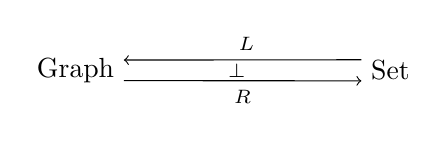
\begin{tikzpicture}
      \node (1) at (0,0) {\( \Graph \)};
      \node (2) at (4,0) {\( \Set \)};
      \node (3) at (2,0) {\scriptsize{ \( \perp \) }};
      \draw [->] (2.160) to node [above] {\scriptsize{ \( L \) }} (1.12);
      \draw [->] (1.-12) to node [below] {\scriptsize{ \( R \) } } (2.-160);
    \end{tikzpicture}
  \]
  %   
  where $ Rx $ is the node set of graph $ x $ and $ La $ is the
  edgeless graph with node set $ a $. An \defn{open graph} is a cospan
  %
  \(
      \csp{La}{x}{Lb}
  \)
  % 
  for sets $ a $, $ b $, and graph $ x $. An illustrated example is
  %
  \[
    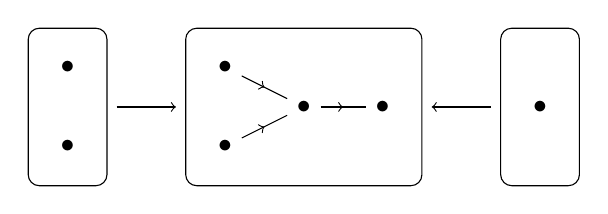
\begin{tikzpicture}
      %
      \begin{scope} % left graph
      \node (1) at (0,1) { \( \bullet \) };
      \node (2) at (0,0) { \( \bullet \) };
      \draw [rounded corners] (-0.5,-0.5) rectangle (0.5,1.5);
      \end{scope}
      %
      \begin{scope}[shift={(2,0)}] % center graph
      \node (1) at (0,1) {\( \bullet \)};
      \node (2) at (0,0) {\( \bullet \)};
      \node (3) at (1,0.5) {\( \bullet  \)};
      \node (4) at (2,0.5) {\( \bullet  \)};
      \draw [->-] (1) to (3);
      \draw [->-] (2) to (3);
      \draw [->-] (3) to (4);
      \draw [rounded corners] (-0.5,-0.5) rectangle (2.5,1.5);
      \end{scope}
      %
      \begin{scope}[shift={(6,0)}] % right graph
      \node (1) at (0,0.5) {\( \bullet \)};
      \draw [rounded corners] (-0.5,-0.5) rectangle (0.5,1.5);
      \end{scope}
      %
      \begin{scope} % graph morphisms
        \node (1) at (0.5,0.5) {};
        \node (2) at (1.5,0.5) {};
        \node (3) at (4.5,0.5) {};
        \node (4) at (5.5,0.5) {};
        \draw [->] (1) to (2);
        \draw [->] (4) to (3);
      \end{scope}
    \end{tikzpicture}
  \]
  % 
  The boxed items are graphs and the arrows between boxes are graph
  morphims defined as suggested by the illustration.  In total, the
  three graphs and two graph morphisms make up a single open graph.   
    
\end{example}

% what good is the open bit?

Having seen this example, it becomes more apparent about how open
systems can ``connect'' together. Given another open graph whose inputs
coincide with the outputs of the graph above, we can connect
the inputs and outputs together to create a new open graph. By passing
from graphs to open graphs, we are introducing
\emph{compositionality}. The category $ \StrCsp\ob $ does not encode
the compositional structure, but we introduce a new category
$ \StrCsp\arr $ in Section \ref{sec:strcsp-as-arrows} for this purpose
and delay further discussion along these lines until then. At present,
we concern ourselves with showing that $ \StrCsp\ob $ is a topos in a
functorial way.  While interesting in itself, this fact allows us to
introduce rewriting systems to structured cospans.

% StrCsp is a topos-valued functor

\begin{theorem} \label{thm:strcsp-istopos}

  The category $ \StrCsp\ob $ is a topos.
  
\end{theorem}

\begin{proof}

  The category $ \StrCsp\ob $ constructed using the adjunction
  $ L \dashv R \from \A \to \X $ is equivalent to the category
  whose objects are cospans of form
  %
  \(
      \csp{a}{Rx}{b}
  \)
  % 
  and morphisms are triples $ ( f,g,h ) $ fitting into the commuting
  diagram
  %
  \[
    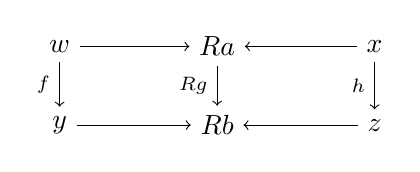
\begin{tikzpicture}
      \node (1) at (-2,1) {\( w \)};
      \node (2) at (0,1) {\( Ra \)};
      \node (3) at (2,1) {\( x \)};
      \node (4) at (-2,0) {\( y \)};
      \node (5) at (0,0) {\( Rb \)};
      \node (6) at (2,0) {\( z \)};
      \draw [->] (1) to  node [] {\scriptsize{\(  \)}} (2);
      \draw [->] (3) to node [] {\scriptsize{\(  \)}} (2);
      \draw [->] (4) to node [] {\scriptsize{\(  \)}} (5);
      \draw [->] (6) to node [] {\scriptsize{\(  \)}} (5);
      \draw [->] (1) to node [left] {\scriptsize{\( f \)}} (4);
      \draw [->] (2) to node [left] {\scriptsize{\( Rg \)}} (5);
      \draw [->] (3) to node [left] {\scriptsize{\( h \)}} (6); 
    \end{tikzpicture}
  \]
  % 
  This, in turn, is equivalent to the comma category
  $ ( \X \downarrow \Delta R ) $, where
  $ \Delta \from \X \to \X \times \X $ is the diagonal functor. But
  the diagonal functor is right adjoint to taking binary
  products. That means $ \Delta R $ is also a right adjoint and,
  furthermore that $ ( X \downarrow \Delta X ) $ is an instance of
  Artin glueing,
  %
  \todo{CITE ARTIN GLUEING}
   hence a topos.

\end{proof}

Until now, the topos $ \StrCsp\ob $ depended on an adjunction fixed at
the beginning of the section.  By letting the adjunction vary, we see
that $ \StrCsp\ob $ is actually functorial.

For the following theorem, denote by $ \Topos $ the category of
elementary topoi and geometric morphisms.

\begin{theorem} \label{thm:strcsp-isfunctorial}

  There is a functor
  %
  \[
    \StrCsp\ob \from
    [ \bullet \to \bullet , \Topos ]
    \to
    \Topos
  \]
  % 
  defined by  
  \[
    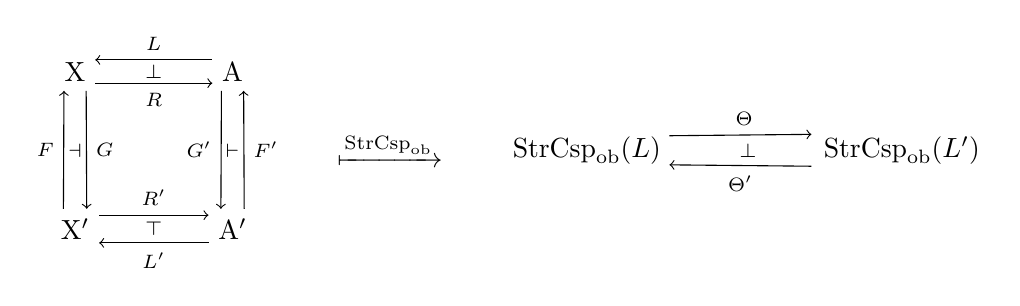
\begin{tikzpicture}
      \begin{scope}
      \node (1) at (-1,1) {\( \X \)};
      \node (2) at (-1,-1) {\( \X' \)};
      \node (3) at (1,1) {\( \A \)};
      \node (4) at (1,-1) {\( \A' \)};
      \draw [->] (1.-60) to node [right] {\scriptsize{\( G \)}} (2.60);
      \draw [<-] (1.-120) to node [left] {\scriptsize{\( F \)}} (2.120);
      \draw [<-] (1.30) to node [above] {\scriptsize{\( L \)}} (3.150);  
      \draw [->] (1.-30) to node [below] {\scriptsize{\( R \)}} (3.-150);
      \draw [->] (2.30) to node [above] {\scriptsize{\( R' \)}} (4.150);
      \draw [<-] (2.-30) to node [below] {\scriptsize{\( L' \)}} (4.-150);      
      \draw [<-] (3.-60) to node [right] {\scriptsize{\( F' \)}} (4.60);
      \draw [->] (3.-120) to node [left] {\scriptsize{\( G' \)}}
      (4.120);
      \node (5) at (0,-1) {\scriptsize{\( \top \)}};
      \node (6) at (0,1) {\scriptsize{\( \perp \)}};
      \node (7) at (-1,0) {\scriptsize{\( \dashv \)}};
      \node (8) at (1,0) {\scriptsize{\( \vdash \)}};
      \end{scope}
     % 
      \begin{scope}[shift={(3,0)}]
      \node (1) at (0,0) { $\xmapsto{ \StrCsp\ob }$ };
      \end{scope}
      %
      \begin{scope}[shift={(5.5,0)}]
      \node (1) [inner sep=0.1cm] at (0,0) {\( \StrCsp\ob (L) \)};
      \node (2) [inner sep=0.15cm] at (4,0) {\( \StrCsp\ob (L') \)};
      \node (3) at (2,0) {\scriptsize{ \( \perp \) }};
      \draw [->] (1.10) to node [above] {\scriptsize{ \( \Theta \) }} (2.170);
      \draw [->] (2.-170) to node [below] {\scriptsize{ \( \Theta' \) } } (1.-10);  
      \end{scope}
    \end{tikzpicture}
  \]
  % 
  which is in turn given by
  %
  \[
    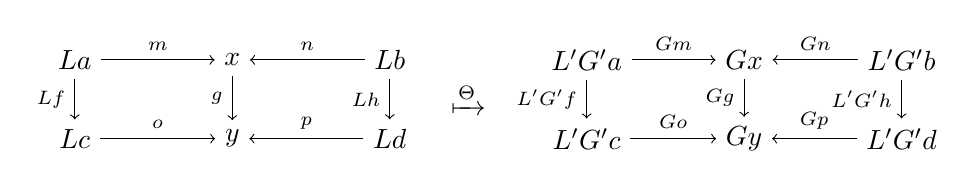
\begin{tikzpicture}
      \begin{scope}
      \node (1) at (-2,1) {\( La \)};
      \node (2) at (0,1) {\( x \)};
      \node (3) at (2,1) {\( Lb \)};
      \node (4) at (-2,0) {\( Lc \)};
      \node (5) at (0,0) {\( y \)};
      \node (6) at (2,0) {\( Ld \)};
      \draw [->] (1) to node [above] {\scriptsize{\( m \)}} (2);
      \draw [->] (3) to node [above] {\scriptsize{\( n \)}} (2);
      \draw [->] (4) to node [above] {\scriptsize{\( o \)}} (5);
      \draw [->] (6) to node [above] {\scriptsize{\( p \)}} (5);
      \draw [->] (1) to node [left] {\scriptsize{\( Lf \)}} (4);
      \draw [->] (2) to node [left] {\scriptsize{\( g \)}} (5);
      \draw [->] (3) to node [left] {\scriptsize{\( Lh \)}} (6);
      \end{scope}
      %
      \begin{scope}[shift={(3,0)}]
      \node (1) at (0,0.5) { $ \xmapsto{ \Theta } $ };
      \end{scope}
      %
      \begin{scope}[shift={(6.5,0)}]
      \node (1) at (-2,1) {\( L'G'a \)};
      \node (2) at (0,1) {\( Gx \)};
      \node (3) at (2,1) {\( L'G'b \)};
      \node (4) at (-2,0) {\( L'G'c \)};
      \node (5) at (0,0) {\( Gy \)};
      \node (6) at (2,0) {\( L'G'd \)};
      \draw [->] (1) to node [above] {\scriptsize{\( Gm \)}} (2);
      \draw [->] (3) to node [above] {\scriptsize{\( Gn \)}} (2);
      \draw [->] (4) to node [above] {\scriptsize{\( Go \)}} (5);
      \draw [->] (6) to node [above] {\scriptsize{\( Gp \)}} (5);
      \draw [->] (1) to node [left] {\scriptsize{\( L'G'f \)}} (4);
      \draw [->] (2) to node [left] {\scriptsize{\( Gg \)}} (5);
      \draw [->] (3) to node [left] {\scriptsize{\( L'G'h \)}} (6);  
      \end{scope}
    \end{tikzpicture}
  \]
  %
  and
  \[
    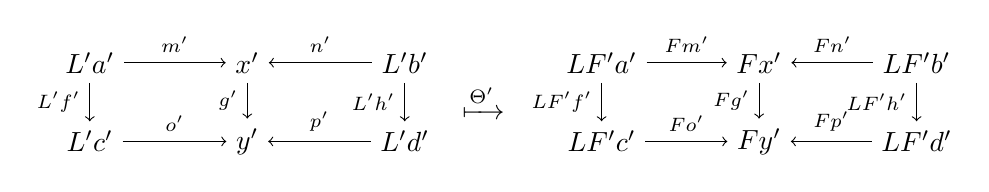
\begin{tikzpicture}
      \begin{scope}
      \node (1) at (-2,1) {\( L'a' \)};
      \node (2) at (0,1) {\( x' \)};
      \node (3) at (2,1) {\( L'b' \)};
      \node (4) at (-2,0) {\( L'c' \)};
      \node (5) at (0,0) {\( y' \)};
      \node (6) at (2,0) {\( L'd' \)};
      \draw [->] (1) to node [above] {\scriptsize{\( m' \)}} (2);
      \draw [->] (3) to node [above] {\scriptsize{\( n' \)}} (2);
      \draw [->] (4) to node [above] {\scriptsize{\( o' \)}} (5);
      \draw [->] (6) to node [above] {\scriptsize{\( p' \)}} (5);
      \draw [->] (1) to node [left] {\scriptsize{\( L'f' \)}} (4);
      \draw [->] (2) to node [left] {\scriptsize{\( g' \)}} (5);
      \draw [->] (3) to node [left] {\scriptsize{\( L'h' \)}} (6);
      \end{scope}
      %
      \begin{scope}[shift={(3,0)}]
      \node (1) at (0,0.5) { $ \xmapsto{ \Theta' } $ };
      \end{scope}
      %
      \begin{scope}[shift={(6.5,0)}]
      \node (1) at (-2,1) {\( LF'a' \)};
      \node (2) at (0,1) {\( Fx' \)};
      \node (3) at (2,1) {\( LF'b' \)};
      \node (4) at (-2,0) {\( LF'c' \)};
      \node (5) at (0,0) {\( Fy' \)};
      \node (6) at (2,0) {\( LF'd' \)};
      \draw [->] (1) to node [above] {\scriptsize{\( Fm' \)}} (2);
      \draw [->] (3) to node [above] {\scriptsize{\( Fn' \)}} (2);
      \draw [->] (4) to node [above] {\scriptsize{\( Fo' \)}} (5);
      \draw [->] (6) to node [above] {\scriptsize{\( Fp' \)}} (5);
      \draw [->] (1) to node [left] {\scriptsize{\( LF'f' \)}} (4);
      \draw [->] (2) to node [left] {\scriptsize{\( Fg' \)}} (5);
      \draw [->] (3) to node [left] {\scriptsize{\( LF'h' \)}} (6);  
      \end{scope}
    \end{tikzpicture}
  \]  
\end{theorem}

\begin{proof}

  In light of Lemma \ref{thm:strcsp-istopos}, it suffices to show that
  $ \Theta \dashv \Theta' $ gives a geometric morphism.

  Denote the structured cospans
  %
  \[
    La \xto{m} x \xgets{n} Lb
  \]
  % 
  in $ \StrCsp\ob ( L ) $ by   
  %
  \[
    L'a' \xto{m'} x' \xgets{n'} L'b'
  \]
  % 
  in $ \StrCsp\ob ( L' ) $ by $ \ell $ and $ \ell' $,
  respectively. Also, denote the unit and counit for $F \dashv G$ by
  $ \eta $, $ \varepsilon $ and for $ F' \dashv G' $ by $ \eta' $, $
  \varepsilon' $.  The assignments
  %
  \begin{align}
    \left(
      ( f,g,h ) \from \ell \to \Theta' \ell'
      \right)
    & \mapsto
    \left(
      ( \varepsilon' \circ F'f , \varepsilon \circ Fg , \varepsilon'
      \circ F'h )
      \from \Theta \ell \to \ell'
      \right) \\
      %
      \left(
      ( f',g',h' ) \from \Theta \ell \to \ell'
      \right)
    & \mapsto
      \left(
      ( G'f' \circ \eta', Gg' \circ \eta , G'h' \circ \eta' )
      \from \ell \to \Theta' \ell'
      \right) \\
  \end{align}
  give a bijection $ \hom ( \Theta \ell , \ell' ) \simeq \hom ( \ell ,
  \Theta' \ell' ) $. Moreover, it is natural in $ \ell $ and $ \ell'
  $. This rests on the natural maps $ \eta $, $ \varepsilon $, $ \eta'
  $, and $ \varepsilon' $. The left adjoint $ \Theta' $ preserves
  finite limits because they are taken pointwise and $ L $, $ F $, and
  $ F' $ all preserve finite limits.
\end{proof}

Despite $ \StrCsp\ob $ being a functor, we will often let it refer
to some arbitrary image of the functor. Our meaning should be clear
from the context.

\edit{%
  I need notational fixes in this section.  (1) I have StrCsp
  meaning three different things, a category, a functor,
  and...ooops. (2) I also need to define the category of structured
  cospan categories. I don't want to make this a 2-category if I can
  help it.  The maps between structured cospan cats should be pairs of
  functors strictly commuting with the boundary and interior of the
  structured cospans.  Also, even though the category of structured
  cospans is a subcat of Topos, I don't actually want the functors to
  be geometric morphisms.  Where should I define this category?
}

Even though a structured cospan category is actually a topos, and its
information is drawn from a geometric morphism of topoi, the morphims
between structured cospan categories that we are interested in do not
involve geometric morphisms at all. Given a pair of geometric morphisms from
%
\[
  \adjunction{\X}{L}{R}{\A}
  \quad
  \t{ and }
  \quad
  \adjunction{\X}{L'}{R'}{\A'}
\]
% 
a \defn{structured cospan functor}
%
\[
  \StrCsp\ob (L) \to \StrCsp\ob (L')
\]
% 
consists of a a pair of functors $ F \from \X \to \X' $ and $ G \from
\A \to \A' $ such that $ FL=L'F $ and $ GR = R'F $.  Of course,
structured cospan categories and their morphisms form a category, but
we leave it unnamed.

% ~~~~~~~~~~~~~~~~~~~~~~~~~~~~~~~~~~~~~~~~
% ~~~~~~~~~~~~~~~~~~~~~~~~~~~~~~~~~~~~~~~~
% ~~~~~~~~~~~~~~~~~~~~~~~~~~~~~~~~~~~~~~~~
% ~~~~~~~~~~~~~~~~~~~~~~~~~~~~~~~~~~~~~~~~

\subsection{Structured cospans as morphisms}
\label{sec:strcsp-as-arrows}

We now turn to capturing the compositional structure that
truly motivates the invention of structured cospans.  To do this, we
shift perspectives of structured cospans as objects in $ \StrCsp\ob $
to structured cospans as morphisms, which of course, are composable. 

Continue to fix a geometric morphism $ L \dashv R \from
\X \to \A $.

\begin{definition} \label{def:strcsp-arr}
  
  Denote by $ \StrCsp\arr $ the category that has the same objects as
  $ \A $ and structured cospans $ \csp{La}{x}{Lb} $ as arrows of
  type $ a \to b $.
  
\end{definition}

Note that composition is defined by pushout:
%
\[
  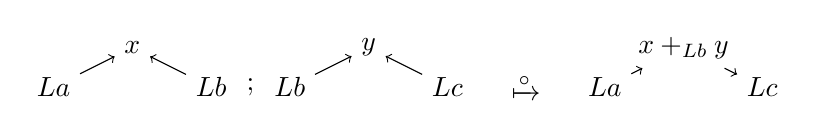
\begin{tikzpicture}
    \begin{scope}
    \node (1) at (0,0) {\( La \)};
    \node (2) at (1,0.5) {\( x \)};
    \node (3) at (2,0) {\( Lb \)};
    \node (4) at (3,0) {\( Lb \)};
    \node (5) at (4,0.5) {\( y \)};
    \node (6) at (5,0) {\( Lc \)};
    \node (7) at (2.5,0) {\( ; \)};
    \draw [->] (1) to node [] {\scriptsize{\(  \)}} (2);
    \draw [->] (3) to node [] {\scriptsize{\(  \)}} (2);
    \draw [->] (4) to node [] {\scriptsize{\(  \)}} (5);
    \draw [->] (6) to node [] {\scriptsize{\(  \)}} (5);
    \end{scope}
    %
    \begin{scope}[shift={(6,0)}]
    \node (1) at (0,0) {\( \xmapsto{\circ} \)};
    \end{scope}
    %
    \begin{scope}[shift={(7,0)}]
    \node (1) at (0,0) {\( La \)};
    \node (2) at (1,0.5) {\( x +_{Lb} y \)};
    \node (3) at (2,0) {\( Lc \)};
     \draw [->] (1) to node [] {\scriptsize{\(  \)}} (2);
    \draw [->] (2) to node [] {\scriptsize{\(  \)}} (3); 
    \end{scope}
  \end{tikzpicture}
\]
% 

Pushouts, in a sense, are a way of glueing things
together. Composition as using pushouts is sensible to model
system connection; we have two systems
%
\[
  \csp{La}{x}{Lb}
  \t{ and}
  \csp{Lb}{y}{Lc}
\]
% 
whose composition is like connecting them along the common interface
$ Lb $. To illustrate how the structured cospan formalism allows us to connect
systems together, we return to the open graphs example.

\begin{example} \label{ex:open-graph-as-arrow}

  The open graph
  % 
  \[
    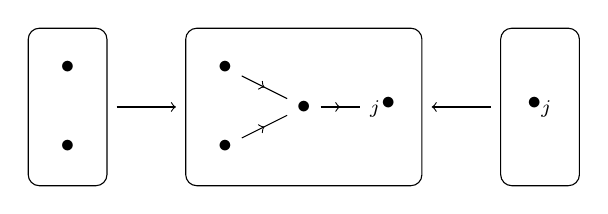
\begin{tikzpicture}
       %
      \begin{scope} % left graph
      \node (1) at (0,1) { \( \bullet \) };
      \node (2) at (0,0) { \( \bullet \) };
      \draw [rounded corners] (-0.5,-0.5) rectangle (0.5,1.5);
      \end{scope}
      %
      \begin{scope}[shift={(2,0)}] % center graph
      \node (1) at (0,1) {\( \bullet \)};
      \node (2) at (0,0) {\( \bullet \)};
      \node (3) at (1,0.5) {\( \bullet  \)};
      \node (4) at (2,0.5) {\( {}_{j} \bullet  \)};
      \draw [->-] (1) to (3);
      \draw [->-] (2) to (3);
      \draw [->-] (3) to (4);
      \draw [rounded corners] (-0.5,-0.5) rectangle (2.5,1.5);
      \end{scope}
      %
      \begin{scope}[shift={(6,0)}] % right graph
      \node (1) at (0,0.5) {\( \bullet_{j} \)};
      \draw [rounded corners] (-0.5,-0.5) rectangle (0.5,1.5);
      \end{scope}
      %
      \begin{scope} % graph morphisms
      \node (1) at (0.5,0.5) {};
      \node (2) at (1.5,0.5) {};
      \node (3) at (4.5,0.5) {};
      \node (4) at (5.5,0.5) {};
      \draw [->] (1) to (2);
      \draw [->] (4) to (3);
      \end{scope}
      %
    \end{tikzpicture}
  \]
  % 
  can be composed with the open graph
   %
  \[
    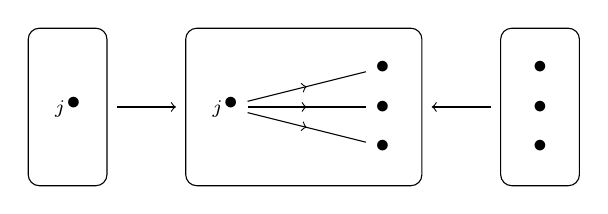
\begin{tikzpicture}
       %
      \begin{scope} % left graph
      \node (1) at (0,0.5) { \( {}_{j} \bullet \) };
      \draw [rounded corners] (-0.5,-0.5) rectangle (0.5,1.5);
      \end{scope}
      %
      \begin{scope}[shift={(2,0)}] % center graph
      \node (1) at (0,0.5) {\( {}_{j} \bullet \)};
      \node (2) at (2,0) {\( \bullet \)};
      \node (3) at (2,0.5) {\( \bullet  \)};
      \node (4) at (2,1) {\( \bullet  \)};
      \draw [->-] (1) to (2);
      \draw [->-] (1) to (3);
      \draw [->-] (1) to (4);
      \draw [rounded corners] (-0.5,-0.5) rectangle (2.5,1.5);
      \end{scope}
      %
      \begin{scope}[shift={(6,0)}] % right graph
      \node (2) at (0,0) {\( \bullet \)};
      \node (3) at (0,0.5) {\( \bullet  \)};
      \node (4) at (0,1) {\( \bullet  \)};
      \draw [rounded corners] (-0.5,-0.5) rectangle (0.5,1.5);
      \end{scope}
      %
      \begin{scope} % graph morphisms
      \node (1) at (0.5,0.5) {};
      \node (2) at (1.5,0.5) {};
      \node (3) at (4.5,0.5) {};
      \node (4) at (5.5,0.5) {};
      \draw [->] (1) to (2);
      \draw [->] (4) to (3);
      \end{scope}
      %
    \end{tikzpicture}
  \]
  %
  to obtain
   %
  \[
    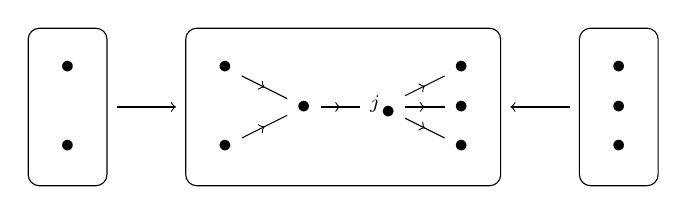
\begin{tikzpicture}
       %
      \begin{scope} % left graph
      \node (1) at (0,1) { \( \bullet \) };
      \node (2) at (0,0) { \( \bullet \) };
      \draw [rounded corners] (-0.5,-0.5) rectangle (0.5,1.5);
      \end{scope}
      %
      \begin{scope}[shift={(2,0)}] % center graph
      \node (1) at (0,1) {\( \bullet \)};
      \node (2) at (0,0) {\( \bullet \)};
      \node (3) at (1,0.5) {\( \bullet  \)};
      \node (4) at (2,0.5) {\( {}^{j} \bullet  \)};
      \node (5) at (3,0) {\( \bullet \)};
      \node (6) at (3,0.5) {\( \bullet  \)};
      \node (7) at (3,1) {\( \bullet  \)};
      \draw [->-] (1) to (3);
      \draw [->-] (2) to (3);
      \draw [->-] (3) to (4);
      \draw [->-] (4) to (5);
      \draw [->-] (4) to (6);
      \draw [->-] (4) to (7);
      \draw [rounded corners] (-0.5,-0.5) rectangle (3.5,1.5);
      \end{scope}
      %
      \begin{scope}[shift={(7,0)}] % right graph
      \node (2) at (0,0) {\( \bullet \)};
      \node (3) at (0,0.5) {\( \bullet  \)};
      \node (4) at (0,1) {\( \bullet  \)};
      \draw [rounded corners] (-0.5,-0.5) rectangle (0.5,1.5);
      \end{scope}
      %
      \begin{scope} % graph morphisms
      \node (1) at (0.5,0.5) {};
      \node (2) at (1.5,0.5) {};
      \node (3) at (5.5,0.5) {};
      \node (4) at (6.5,0.5) {};
      \draw [->] (1) to (2);
      \draw [->] (4) to (3);
      \end{scope}
      %
    \end{tikzpicture}
  \]
  %
  This composition glued the two open graphs together along the node $
  j $.
  
\end{example}

% ~~~~~~~~~~~~~~~~~~~~~~~~~~~~~~~~~~~~~~~~
% ~~~~~~~~~~~~~~~~~~~~~~~~~~~~~~~~~~~~~~~~

\subsection{A bicategory of structured cospans}
\label{sec:bicat-strcsp}

Using bicategories allows us to combine into a single instrument the
competing perspectives of structured cospans as objects and as
morphisms. In this section, we build two bicategories: one to combine
our two perspectives on structured cospans and the other, which comes
in two flavors, anticipates the rewriting contained in Section
\ref{sec:rewriting-strcsp}. Many of the details of these
constructions are already contained in other work, so we will focus
on the ideas and point to the proofs as needed.

Because we the ingredients for our constructions come from a geometric
morphism, there is an implicit cocartesian structure on the topoi
involved. This cocartesianness can be lifted up to the bicategories,
but checking all of the axiom is a tedious process. Instead, we will
rely on a result of Shulman
%
\todo{cite{shulman-constructing}}
%
and build
cocartesian double categories instead of bicategories. The relevant
axioms are much easier to check. Shulman's result then allows us to
chisel the cocartesian double category down to a cocartesian
bicategory. The reason that we prefer bicategories to double
categories is that they are more familar objects with which to work
and the information lost in passing from double to bicategory, in our
case, is minimal.

For a precise definition of a symmetric monoidal double category, we
point to Shulman,
%
\todo{cite{shulman-constructing}}
%
though for the sake of completeness, here are the key ingredients. A
double category $ \CCC $ consists of a pair of categories
$ ( \C_0 , \C_1 ) $ with some additional data that binds them
together, which we ignore. The pieces of the two categories become the
following in the double category:
%
\begin{itemize}
\item the $ \CCC $-\emph{objects} are exactly $ \C_0 $-the objects,
\item the $ \CCC $-\emph{vertical arrows} $ c \to d $ between $ \C
  $-objects are exactly the $ \C_0 $ arrows, 
\item the $ \CCC $-\emph{horizontal arrows} $ c \nrightarrow d $
  between $ \CCC $-objects are the $ \C_1 $-objects together with some
  structure maps assigning the domain and codomain, and
\item the \emph{squares} of $ \CCC $ are
\[
  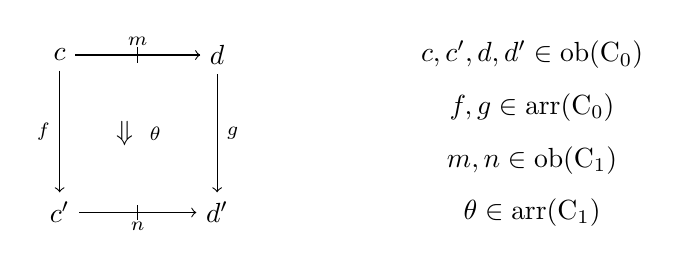
\begin{tikzpicture}
    \node (1) at (0,2) {\( c \)};
    \node (2) at (2,2) {\( d \)};
    \node (3) at (0,0) {\( c' \)};
    \node (4) at (2,0) {\( d' \)};
    \draw [-|->] (1) to node [above] {\scriptsize{\( m \)}} (2);
    \draw [->] (1) to node [left] {\scriptsize{\( f \)}} (3);
    \draw [->] (2) to node [right] {\scriptsize{\( g \)}} (4);
    \draw [-|->] (3) to node [below] {\scriptsize{\( n \)}} (4);
    \node (5) at (6,2) {\( c,c',d,d' \in \operatorname{ob} ( \C_0 ) \)};
    \node (6) at (6,1.33) {\( f,g \in \operatorname{arr} ( \C_0 ) \)};
    \node (7) at (6,.66) {\( m,n \in \operatorname{ob} ( \C_1 ) \)};
    \node (8) at (1,1) {\( \Downarrow \) \scriptsize{ \( \theta \)}};
    \node (9) at (6,0) {\( \theta \in \operatorname{arr} ( \C_1 ) \)};
  \end{tikzpicture}
\]
are the arrows of $ \C_1 $ together with structure maps attaching the
surrounding vertical arrows. 
\end{itemize}
%
The vertical arrows compose as they do in $ \C_0 $ and there are
structure maps that introduce a composition for the horizontal
arrows. The $ 2 $-arrows can compose horizontally and vertically.

We say that a $ 2 $-arrow between identity vertical arrows is
\defn{globular}.  Inside every double category $ \CCC $ is a bicategory
$ H ( \CCC ) $ comprised of the objects, horizontal arrows, and
globular $ 2 $-arrows of $ \CCC $. 

Observe that the horizontal arrows play a dual role, as
objects in their origin category and arrows in the double
category. This reflects the dual perspective on structured cospans.

Now, let us define the first cocartesian bicategory, via a cocartesian
double category.

The first double category that we define is also contained in the
related work by Baez and Courser
%
\todo{CITE COR 3.9 BAEZ COURSER STRCSP}
%
. There, they prove that it actually is
a double category, so we content ourselves to simply provide the
definition.

\begin{definition}

  There is a cocartesian double category
  $ \SSStrCsp \coloneqq ( \A , \StrCsp\ob ) $ :
  \begin{itemize}
  \item the objects are all $ \A $-objects
  \item the vertical arrows $ a \to b $ all $ \A $-arrows, 
  \item the horizontal arrows $ \horarrow{a}{b} $ are
    $ \StrCsp\ob $-objects, that is cospans $ \csp{La}{x}{Lb} $, and
  \item the squares are commuting diagrams
    %
    \[
    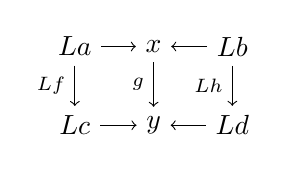
\begin{tikzpicture}
    \node (1) at (0,1) {\( La \)};
    \node (2) at (1,1) {\( x \)};
    \node (3) at (2,1) {\( Lb \)};
    \node (4) at (0,0) {\( Lc \)};
    \node (5) at (1,0) {\( y \)};
    \node (6) at (2,0) {\( Ld \)};
    \draw [->] (1) to node [] {\scriptsize{\(   \)}} (2);
    \draw [->] (3) to node [] {\scriptsize{\(  \)}} (2);
    \draw [->] (4) to node [] {\scriptsize{\(  \)}} (5);
    \draw [->] (6) to node [] {\scriptsize{\(  \)}} (5);
    \draw [->] (1) to node [left] {\scriptsize{\( Lf \)}} (4);
    \draw [->] (2) to node [left] {\scriptsize{\( g \)}} (5);
    \draw [->] (3) to node [left] {\scriptsize{\( Lh \)}} (6);
    \end{tikzpicture}
  \]
  %
 \end{itemize}

  The tensor is pointwise application of the coproduct
  %
  \[
    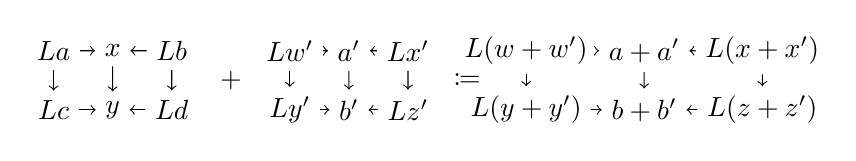
\begin{tikzpicture}[scale=0.75]
      %
      \begin{scope}
      \node (1) at (0,1) {\( La \)};
      \node (2) at (1,1) {\( x \)};
      \node (3) at (2,1) {\( Lb \)};
      \node (4) at (0,0) {\( Lc \)};
      \node (5) at (1,0) {\( y \)};
      \node (6) at (2,0) {\( Ld \)};
      \draw [->] (1) to node [above] {\scriptsize{\(   \)}} (2);
      \draw [->] (3) to node [left] {\scriptsize{\(  \)}} (2);
      \draw [->] (4) to node [right] {\scriptsize{\(  \)}} (5);
      \draw [->] (6) to node [below] {\scriptsize{\(  \)}} (5);
      \draw [->] (1) to node [below] {\scriptsize{\(  \)}} (4);
      \draw [->] (2) to node [below] {\scriptsize{\(  \)}} (5);
      \draw [->] (3) to node [below] {\scriptsize{\(  \)}} (6);   
      \end{scope}
      %
      \begin{scope}[shift={(3,0)}]
      \node (1) at (0,0.5) {$ + $};  
      \end{scope}
      %
      \begin{scope}[shift={(4,0)}]
      \node (1) at (0,1) {\( Lw' \)};
      \node (2) at (1,1) {\( a' \)};
      \node (3) at (2,1) {\( Lx' \)};
      \node (4) at (0,0) {\( Ly' \)};
      \node (5) at (1,0) {\( b' \)};
      \node (6) at (2,0) {\( Lz' \)};
      \draw [->] (1) to node [above] {\scriptsize{\(   \)}} (2);
      \draw [->] (3) to node [left] {\scriptsize{\(  \)}} (2);
      \draw [->] (4) to node [right] {\scriptsize{\(  \)}} (5);
      \draw [->] (6) to node [below] {\scriptsize{\(  \)}} (5);
      \draw [->] (1) to node [below] {\scriptsize{\(  \)}} (4);
      \draw [->] (2) to node [below] {\scriptsize{\(  \)}} (5);
      \draw [->] (3) to node [below] {\scriptsize{\(  \)}} (6);   
      \end{scope}
      %
      \begin{scope}[shift={(7,0)}]
      \node (1) at (0,0.5) {$ \coloneqq $};  
      \end{scope}
      %
      \begin{scope}[shift={(8,0)}]]
      \node (1) at (0,1) {\( L ( w + w' ) \)};
      \node (2) at (2,1) {\( a + a' \)};
      \node (3) at (4,1) {\( L ( x + x' ) \)};
      \node (4) at (0,0) {\( L ( y + y' ) \)};
      \node (5) at (2,0) {\( b + b' \)};
      \node (6) at (4,0) {\( L ( z + z' ) \)};
      \draw [->] (1) to node [above] {\scriptsize{\(   \)}} (2);
      \draw [->] (3) to node [left] {\scriptsize{\(  \)}} (2);
      \draw [->] (4) to node [right] {\scriptsize{\(  \)}} (5);
      \draw [->] (6) to node [below] {\scriptsize{\(  \)}} (5);
      \draw [->] (1) to node [below] {\scriptsize{\(  \)}} (4);
      \draw [->] (2) to node [below] {\scriptsize{\(  \)}} (5);
      \draw [->] (3) to node [below] {\scriptsize{\(  \)}} (6);   
      \end{scope}
    \end{tikzpicture}
  \]  
\end{definition}

As mentioned above, we prefer to work with symmetric monoidal bicategories and use double
categories as a convenient way to arrive there.  Courser
%
\todo{CITE COURSER STR-CSP, COR 3.10}
%
has already proved that the \emph{horizontal bicategory} of $ \SSStrCsp
$ exists, and so we simply describe it.

\begin{definition}

  There is a symmetric monoidal bicategory $ \SStrCsp $ consisting of
  \begin{itemize}
  \item $ \A $-objects for objects,
  \item structured cospans $ \csp{La}{x}{Lb} $ as arrows of type $ a
    \to b $, and
  \item maps of cospans as 2-arrows.    
  \end{itemize}
  
\end{definition}

% ~~~~~~~~~~~~~~~~~~~~~~~~~~~~~~~~~~~~
% ~~~~~~~~~~~~~~~~~~~~~~~~~~~~~~~~~~~~
% ~~~~~~~~~~~~~~~~~~~~~~~~~~~~~~~~~~~~
% ~~~~~~~~~~~~~~~~~~~~~~~~~~~~~~~~~~~~

\section{Rewriting structured cospans}
\label{sec:rewriting-strcsp}

At this point, we have discussed structured cospans enough to begin
the transition to rewriting structured cospans. This and the next
subsection introduce the bicategories that will serve as the ambient
bicategories in which rewriting occurs.  The appropriate style of
rewriting that we on structured cospans is called double pushout (DPO)
rewriting. In this section, we will briefly cover the basics of DPO
rewriting and see how this translates to structured cospans.

A \defn{rewriting system}, in its most general form, is a set $ S $
together with a binary relation $ \rel $. The idea is that
if $ s \rel r$, then $ s $ can be ``replaced'' by $ r
$. This is such a simple framework that, naturally, it has occured in
diverse areas of study and has many different manifestations.  After
Ehrig, et. al.
%
\todo{CITE ERHIG GRAPH TRANSFORM}
%
introduced graph rewriting, Lack and Sobocinski axiomatized it when
they introduced \emph{adhesive categories},
%
\todo{CITE LACK/SOBO ADHESIVE CATS}
%
a place in which one can develop well-behaved double pushout rewriting
systems. This is precisely what we plan to do with structured
cospans. After a recalling the basics of DPO rewriting in adhesive
categories, we introduce the rewriting theory of structured cospans.

While a rewriting system often begins with a set, we begin with an
adhesive category.  Adhesivity is an exactness condition that ensures
certain pushouts behave as they do in $ \Set $. This is captured by
sayin that the pushout satifies the \defn{Van Kampen condition}, which
states that, given a commuting cube
%
\[
  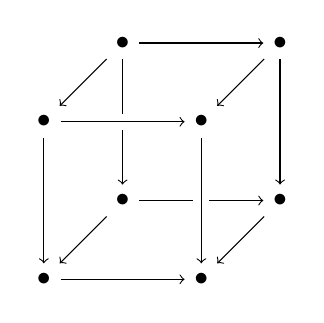
\begin{tikzpicture}
    \node (1) at (1,3) {\( \bullet \)};
    \node (2) at (0,2) {\( \bullet \)};
    \node (3) at (3,3) {\( \bullet \)};
    \node (4) at (2,2) {\( \bullet \)};
    \node (5) at (1,1) {\( \bullet \)};
    \node (6) at (0,0) {\( \bullet \)};
    \node (7) at (3,1) {\( \bullet \)};
    \node (8) at (2,0) {\( \bullet \)};
    \draw [->] (1) to node [] {\scriptsize{\(  \)}} (5);
    \draw [->] (1) to node [] {\scriptsize{\(  \)}} (2);
    \draw [->] (1) to node [] {\scriptsize{\(  \)}} (3);
    \draw [white, line width=2mm] (2) -- (4);
    \draw [->] (2) to node [] {\scriptsize{\(  \)}} (4);
    \draw [->] (3) to node [] {\scriptsize{\(  \)}} (4);
    \draw [->] (5) to node [] {\scriptsize{\(  \)}} (6);
    \draw [->] (5) to node [] {\scriptsize{\(  \)}} (7);
    \draw [->] (6) to node [] {\scriptsize{\(  \)}} (8);
    \draw [->] (7) to node [] {\scriptsize{\(  \)}} (8);
    \draw [->] (2) to node [] {\scriptsize{\(  \)}} (6);
    \draw [->] (3) to node [] {\scriptsize{\(  \)}} (7);
    \draw [white, line width=2mm] (4) -- (8);
    \draw [->] (4) to node [] {\scriptsize{\(  \)}} (8);
  \end{tikzpicture}
\]
% 
whose bottom face is the pushout and back faces are pullbacks, then
the front faces are pullbacks if and only if the top face is a pushout.

\begin{definition} \label{dfn:adhesive-category} 

  A category with pullbacks is \defn{adhesive} if pushouts along
  monics exist and are \emph{Van Kampen}.

\end{definition} 

An adhesive category is a place where rewrite systems
retain important properties of DPO graph rewriting, namely
concurrency.
%
\todo{cite lack/sobo}
%
While the set component of a rewrite system will come from the objects
of an adhesive category, the binary relation will be given by
\emph{productions}.

\begin{definition}

  A \defn{linear production} $ p $ is a span
  %
  \[
    \ell \leftarrowtail k \rightarrowtail r
  \]
  % 
  with monic legs.  A \defn{left-linear production} is a span whose
  left leg is monic. In cases where a disinction is unimportant, we
  simply write ``production''. 
  
\end{definition}

The way to consider a span in this context is that we are starting
with some object $ \ell $ and replacing it with $ r $, while $ k $
gives the part of $ \ell $ and $ r $ that is fixed throughout the
rewrite.  In the style of DPO rewriting, a rewriting system is often
called a grammar. Specifically a \defn{grammar}
$ G \coloneqq ( \C , P ) $ consists of an adhesive category $ \C $ and
a set of productions $ P $ in $ \C $. The collective feet of the spans
in $ P $ give us the set of objects that forms part of a rewriting
system.  However, this only forms part of the picture, in that a
grammar is really the seed of a rich language.

\begin{definition}
  There is a category $ \Gram $ of consisting of
  \begin{itemize}
  \item grammars $ ( \C , P ) $ as objects, and
  \item as arrows $ ( \C , P ) \to ( \D , Q ) $ are functors $ F \from
    \C \to D $ such that $ FP \subseteq Q $.
  \end{itemize}
\end{definition}

\begin{definition}

  Given a grammar $ G \coloneqq ( \C , P ) $ and a production
  $ p \coloneqq ( \ell \gets k \to r ) $ in $ P $, we say that the
  production $ \spn{\ell'}{k'}{r'} $ is \defn{derived} from $ p $ if
  there is a $ \C $-arrow $ m \from \ell \to D\ell $ fitting into a
  \emph{double pushout} diagram %
  \[
    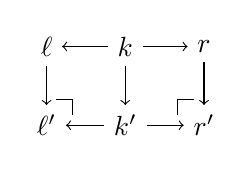
\begin{tikzpicture}
      \node (1) at (0,1) {\( \ell \)};
      \node (2) at (1,1) {\( k \)};
      \node (3) at (2,1) {\( r \)};
      \node (4) at (0,0) {\( \ell' \)};
      \node (5) at (1,0) {\( k' \)};
      \node (6) at (2,0) {\( r' \)};
      \draw [->] (2) to node [] {\scriptsize{\( \)}} (1);
      \draw [->] (2) to node [] {\scriptsize{\( \)}} (3);
      \draw [->] (5) to node [] {\scriptsize{\( \)}} (4);
      \draw [->] (5) to node [] {\scriptsize{\( \)}} (6);
      \draw [->] (1) to node [] {\scriptsize{\( \)}} (4);
      \draw [->] (2) to node [] {\scriptsize{\( \)}} (5);
      \draw [->] (3) to node [] {\scriptsize{\( \)}} (6);
      %
      \node (a) at (0,0.33) {};
      \node (b) at (0.33,0.33) {};
      \node (c) at (0.33,0) {};
      \node (d) at (1.66,0) {};
      \node (e) at (1.66,0.33) {};
      \node (f) at (2,0.33) {};
      \draw (a) -- (b.center);
      \draw (b.center) -- (c);
      \draw (d) -- (e.center);
      \draw (e.center) -- (f);
    \end{tikzpicture}
  \]
  %
  We call the arrow $ m $ a \defn{match} of $ \ell $ in $ \ell' $.
  
  Denote by $ DG $ the grammar consisting of all productions derived
  from $ G $. We will abuse notation slightly and denote by $ DP $ the
  set of productions derived from $ P $. Thus, $ DG $ and $ ( \C , DP
  ) $ refer to the same object in $ \Gram $.
  
\end{definition}

Given a pair of arrows
\[
  \begin{tikzpicture}
    \node (1) at (-1,1) {\( w \)};
    \node (3) at (1,1) {\( y \)};
    \node (4) at (1,-1) {\( d \)};
    \draw [->] (1) to node [above] {\scriptsize{\( \theta \)}} (3);
    \draw [->] (3) to node [right] {\scriptsize{\(  \)}} (4);
  \end{tikzpicture}
\]
that fit into a pushout
\[
  \begin{tikzpicture}
    \node (1) at (-1,1) {\( w \)};
    \node (2) at (-1,-1) {\( x \)};
    \node (3) at (1,1) {\( y \)};
    \node (4) at (1,-1) {\( d \)};
    \draw [->] (1) to node [left] {\scriptsize{\(  \)}} (2);
    \draw [->] (1) to node [above] {\scriptsize{\( \theta \)}} (3);
    \draw [->] (2) to node [above] {\scriptsize{\(  \)}} (4);
    \draw [->] (3) to node [right] {\scriptsize{\(  \)}} (4);
    %
    \node (a) at (0.66,-1) {};
    \node (b) at (0.66,-0.66) {};
    \node (c) at (1,-0.66) {};
    \draw (a) -- (b.center);
    \draw (b.center) -- (c);
  \end{tikzpicture}
\]
we call the object $ x $ the \defn{pushout complement}. If $ \theta $
is monic, then the pushout complement is unique up to isomorphism.
%
\todo{cite lack/sobo}
%
This ensures that a linear or left-linear production together with a
match determine a derived production up to isomorphism. 

This next lemma justifies us naming $ D $ the \defn{derivation
  functor}.

\begin{lemma}
  The construction $ D \from \Gram \to \Gram $ is functorial.
  Moreover
  \begin{enumerate}
  \item $ \id $ on $ \Gram $ is a subfunctor of $ D $,
  \item $ D $ is idempotent
  \item \edit{anything other awesom properties?}
  \end{enumerate}
\end{lemma}

\begin{proof}
  
  \begin{enumerate}
  \item It suffices to find a monic $ G \to DG $ for an arbitrary
    grammar $ G \coloneqq ( \C , P ) $. We claim that the identity
    functor $ \id_{\C} $ gives the monic we seek. Any production is a
    derivation of itself via a triple of identity arrows, and so
    $ \id_{\C} $ gives an arrow $ G \to DG $. It is straighforward to
    check that this is a monic.
  \item This is equivalent to saying that, for a set $ P $ of
    productions, $ DP = DDP $, which follows from the fact that the
    outer box of the diagram
    %
    \[
      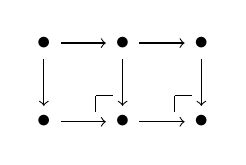
\begin{tikzpicture}
        \node (1) at (0,1) {\( \bullet \)};
        \node (2) at (1,1) {\( \bullet \)};
        \node (3) at (2,1) {\( \bullet \)};
        \node (4) at (0,0) {\( \bullet \)};
        \node (5) at (1,0) {\( \bullet \)};
        \node (6) at (2,0) {\( \bullet \)};
        \draw [->] (1) to node [] {\scriptsize{\(  \)}} (2);
        \draw [->] (2) to node [] {\scriptsize{\(  \)}} (3);
        \draw [->] (4) to node [] {\scriptsize{\(  \)}} (5);
        \draw [->] (5) to node [] {\scriptsize{\(  \)}} (6);
        \draw [->] (1) to node [] {\scriptsize{\(  \)}} (4);
        \draw [->] (2) to node [] {\scriptsize{\(  \)}} (5);
        \draw [->] (3) to node [] {\scriptsize{\(  \)}} (6);
        %
        \node (a) at (0.66,0) {};
        \node (b) at (0.66,0.33) {};
        \node (c) at (1,0.33) {};
        \node (d) at (1.66,0) {};
        \node (e) at (1.66,0.33) {};
        \node (f) at (2,0.33) {};
        \draw (a) -- (b.center);
        \draw (b.center) -- (c);
        \draw (d) -- (e.center);
        \draw (e.center) -- (f);
      \end{tikzpicture}
    \]
    %
    is a pushout.
  \end{enumerate}
  
\end{proof}

Another important functor for us generates a category from a grammar.

\begin{definition} 

  Define a functor $ S \from \Gram \to \Cat $ as follows:
  \begin{itemize}
  \item for a grammar $ G \coloneqq ( \C , P ) $, let $ SG $ be the
    subcategory of $ \Span{ \C } $ generated by the productions in $ P
    $, and
  \item for an arrow of grammars
    $ F \from ( \C , P ) \to ( \D , Q ) $, let $ SF $ be the functor
    given by $ SFc = Fc $ and
    %
    \[
      ( c \xgets{f} d \xto{g} e )
      \mapsto
      ( Fc \xgets{Ff} Fd \xto{Fg} Fe )
    \]
    % 
  \end{itemize}

\end{definition}

In classical rewriting theory, that is when working with a set
together with a binary relation, one is typically more interested in
the transitive and reflexive closure of the relation. This relation
gives for each element of your set, all the possible elements that one
can obtain by successivly applying production rules.  This is in
opposition to the given binary relation which simply gives what one
can obtain by a single application of a production rule.  The functor
$ S \from \Gram \to \Cat $ is the analog of this in our context. 

\begin{theorem}

  A grammar $ G \coloneqq ( \C , P ) $ induces an binary operation
  $ \rel $ on $ P_{\t{feet}} $
  %
  \todo{define this set somewhere and find better notation}
  %
  by $ \ell \rel r $ whenever there is a cospan
  $ \ell \gets k \to r $ in $ P $. Denote by $ \rel^\ast $ the
  transitive and reflexive closure of $ \nrightarrow $. Then $ \ell
  \rel^\ast r $ if and only if there is an arrow $ \ell \to r
  $ in $ SG $.
  
\end{theorem}
 
\begin{proof}

  If $ \ell \rel^\ast r $, then there is a zig-zag from $ \ell
  $ to $ r $ comprised of spans in $ P $ or identity spans.  This
  zig-zag gives a sequence of composable arrows in $ SG $.
  Conversely, if there there is an arrow $ \ell \to r $ in $ SG $,
  then this arrow is a composite of generating arrows, which are
  exactly productions in $ P $.
  
\end{proof}

\begin{definition}

  Define the \defn{language} functor by $ \Lang \coloneqq SD $. In
  particular, given a grammar $ G $, we say that the category $ \Lang
  G $ is the \defn{language of $ G $}.
  
\end{definition}

At this point, the fact that categories of structured cospans are
topoi (cf.~Theorem \ref{thm:strcsp-istopos}) becomes relevant. In
their work on adhesive categories, Lack and Sobocinski proved the
following theorem.  
% 
\todo{cite topos adhesive}
%

\begin{theorem} \label{thm:dpo_topoi-adhesive} 
  Topoi are adhesive.
\end{theorem}

\begin{corollary} \label{thm:dpo_category-StrCsp-adhsv}
  The category $ \StrCsp\ob $ is adhesive.
\end{corollary}

This corollary ensures that we are working within reasonable
constraints to define rewriting of structured cospans. That is, we can
equip a structured cospan category with a set of productions and study
the resulting grammar.

\begin{definition}

  Denote by $ \StrCspGram $ the full subcategry of $ \Gram $
  consisting of grammars $ ( \C , P ) $ such that $ \C $ is a
  structured cospan category.
  
\end{definition}

Restricting $ \Lang $ along the inclusion of $ \StrCspGram $ into
$ \Gram $, we see that assigning the language to a grammar is
functorial even if that grammar is from a structured cospan
category.

To be clear, the language of a grammar of structured cospans
$ \Lang ( \StrCsp\ob (L) , P ) $ is a subcategory of
$ \Span{\StrCsp\ob (L)} $ generated by commuting diagrams of form
%
\[
  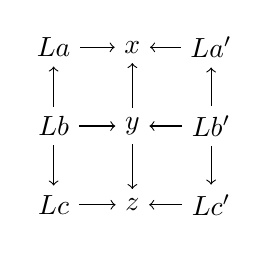
\begin{tikzpicture}
    \node (1) at (0,2) {\( La \)};
    \node (2) at (1,2) {\( x \)};
    \node (3) at (2,2) {\( La' \)};
    \node (4) at (0,1) {\( Lb \)};
    \node (5) at (1,1) {\( y \)};
    \node (6) at (2,1) {\( Lb' \)};
    \node (7) at (0,0) {\( Lc \)};
    \node (8) at (1,0) {\( z \)};
    \node (9) at (2,0) {\( Lc' \)};
    \draw [->] (1) to node [] {\scriptsize{\(  \)}} (2);
    \draw [->] (3) to node [] {\scriptsize{\(  \)}} (2);
    \draw [->] (4) to node [] {\scriptsize{\(  \)}} (5);
    \draw [->] (6) to node [] {\scriptsize{\(  \)}} (5);
    \draw [->] (7) to node [] {\scriptsize{\(  \)}} (8);
    \draw [->] (9) to node [] {\scriptsize{\(  \)}} (8);
    \draw [->] (4) to node [] {\scriptsize{\(  \)}} (1);
    \draw [->] (4) to node [] {\scriptsize{\(  \)}} (7);
    \draw [->] (5) to node [] {\scriptsize{\(  \)}} (2);
    \draw [->] (5) to node [] {\scriptsize{\(  \)}} (8);
    \draw [->] (6) to node [] {\scriptsize{\(  \)}} (3);
    \draw [->] (6) to node [] {\scriptsize{\(  \)}} (9); 
  \end{tikzpicture}
\]
% 
This arrow from $ \csp{La}{x}{La'}$ to $ \csp{Lc}{z}{Lc'} $ is a
composite of spans from $ DP $.

We restrict our attention to structured cospan grammars whose
productions have the form 
\[
  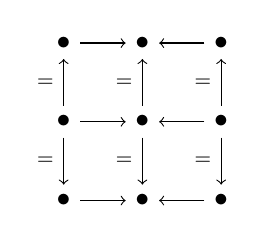
\begin{tikzpicture}
    \node (1) at (0,2) {\( \bullet \)};
    \node (2) at (1,2) {\( \bullet \)};
    \node (3) at (2,2) {\( \bullet \)};
    \node (4) at (0,1) {\( \bullet \)};
    \node (5) at (1,1) {\( \bullet \)};
    \node (6) at (2,1) {\( \bullet \)};
    \node (7) at (0,0) {\( \bullet \)};
    \node (8) at (1,0) {\( \bullet \)};
    \node (9) at (2,0) {\( \bullet \)};
    \draw [->] (1) to node [] {\scriptsize{\(  \)}} (2);
    \draw [->] (3) to node [] {\scriptsize{\(  \)}} (2);
    \draw [->] (4) to node [] {\scriptsize{\(  \)}} (5);
    \draw [->] (6) to node [] {\scriptsize{\(  \)}} (5);
    \draw [->] (7) to node [] {\scriptsize{\(  \)}} (8);
    \draw [->] (9) to node [] {\scriptsize{\(  \)}} (8);
    \draw [->] (4) to node [left] {\scriptsize{\( =  \)}} (1);
    \draw [->] (4) to node [left] {\scriptsize{\( = \)}} (7);
    \draw [->] (5) to node [left] {\scriptsize{\( =  \)}} (2);
    \draw [->] (5) to node [left] {\scriptsize{\( = \)}} (8);
    \draw [->] (6) to node [left] {\scriptsize{\( = \)}} (3);
    \draw [->] (6) to node [left] {\scriptsize{\( = \)}} (9); 
  \end{tikzpicture}
\]
% 
The pragmatic reason is that when rewriting open systems, which we are
formalizing with structured cospans, such productions will ensure that
all morphisms in the language will fix the inputs and
outputs. Another reason is that we actually get a richer structure
when making this restriction: the language is a bicategory, not just a
category.

So far, we have discussed productions without distinguishing between
linear and left-linear productions.  Here is the point where this
distinction becomes important, as the theory of languages for \emph{
  linear grammars} diverges from the theory of \emph{left-linear
  grammars}.

% ~~~~~~~~~~~~~~~~~~~~~~~~~~~~~~~~~~~~
% ~~~~~~~~~~~~~~~~~~~~~~~~~~~~~~~~~~~~
% ~~~~~~~~~~~~~~~~~~~~~~~~~~~~~~~~~~~~
% ~~~~~~~~~~~~~~~~~~~~~~~~~~~~~~~~~~~~

\section{Languages for linear grammars}
\label{sec:lang-linear-grammars}

In this section, we pick up by studying languages for linear grammars,
defined below. In Section \ref{sec:dpo-rewriting}, we showed that the
language of a grammar is the free category generated by arrows coming
from a set of productions. Here we show that the language of a linear
grammar can be structurally richer, depending on the nature of the set
of productions. We begin by constructing a double category valued
language functor. Then we we show that we can actually get a language
that is a symmetric monoidal double category, symmetric monoidal
bicategory, or compact closed bicategory by placing the right
conditions on the grammars.

\begin{definition} \label{def:linear-grammar}

  We say that a grammar $ ( \C , P ) $ is \emph{linear} if
  $ \C \coloneqq \StrCsp ( L ) $ is a structured cospan category and
  the productions in $ P $ are of the form
  %
    \[
      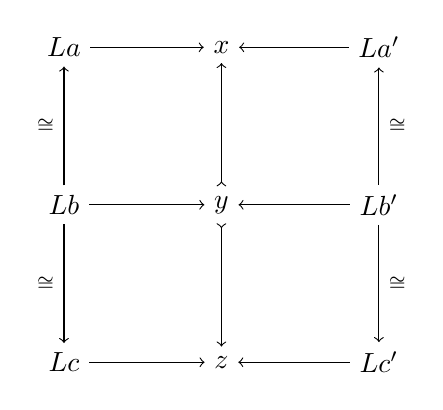
\begin{tikzpicture}
        \begin{scope}
        \node (1) at (0,4) {\( La  \)};
        \node (2) at (2,4) {\( x \)};
        \node (3) at (4,4) {\( La' \)};
        \node (4) at (0,2) {\( Lb \)};
        \node (5) at (2,2) {\( y \)};
        \node (6) at (4,2) {\( Lb' \)};
        \node (7) at (0,0) {\( Lc \)};
        \node (8) at (2,0) {\( z \)};
        \node (9) at (4,0) {\( Lc' \)};
        \draw [->] (1) to node [] {\scriptsize{\(  \)}} (2);
        \draw [->] (3) to node [] {\scriptsize{\(  \)}} (2);
        \draw [->] (4) to node [] {\scriptsize{\(  \)}} (5);
        \draw [->] (6) to node [] {\scriptsize{\(  \)}} (5);
        \draw [->] (7) to node [] {\scriptsize{\(  \)}} (8);
        \draw [->] (9) to node [] {\scriptsize{\(  \)}} (8);
        \draw [->] (4) to node [left] {\scriptsize{\( \iso \)}} (1);
        \draw [->] (4) to node [left] {\scriptsize{\( \iso \)}} (7);
        \draw [>->] (5) to node [] {\scriptsize{\(  \)}} (2);
        \draw [>->] (5) to node [] {\scriptsize{\(  \)}} (8);
        \draw [->] (6) to node [right] {\scriptsize{\( \iso \)}} (3);
        \draw [->] (6) to node [right] {\scriptsize{\( \iso \)}} (9);
        \end{scope}
      \end{tikzpicture}
    \]
    %
    Denote by $ \Gram\lin $ the full subcategory of $ \Gram $ on the
    linear grammars.
  
\end{definition}

There is a reasonable objection to calling such a grammar ``linear''
because we are restricting the adhesive category and the productions
beyond simply linear productions. However, for our purposes,
``linear'' serves as an adequate qualifier.

To avoid a proliferation of large diagrams, we will refer denote a
structured cospan by a single letter as opposed to drawing the
cospan.  This allows us to draw the diagram in Definition
\ref{def:linear-grammar} as a span $ r \gets s \to t $ for structured
cospans $ r $, $ s $, and $ t $. 

Fix a structured cospan category $ \StrCsp\ob (L) $. This is adhesive
and so to choose a set of linear productions $ P $ of these structured
cospans is to give a linear grammar
%
\(
  G \coloneqq ( \StrCsp\ob (L) , P ).
\)
% 
In the previous section, we defined the language functor
%
\(
  \Lang \from \Gram \to \Cat 
\)
% 
that returns the language associated to a grammar. By restricting
grammars to linear grammars we obtain a linear language functor
$ \Lang\lin \from \Gram\lin \to \DblCat $ valued in double categories.
The following lemma ensures that $ \Gram\lin $ is a valid codomain for
this functor.
%
\todo{cite lack-sobo}
%

\begin{lemma} \label{thm:po-respect-monics}
  
  In an adhesive category, pushouts respect monics.

\end{lemma}

This lemma, together with the fact that topoi are regular categories, ensure that the restriction of the derivation functor to $
\Gram\lin $ returns a linear grammar. Indeed, double pushout diagram
in $ \StrCsp (L) $ looks like
%
\[
  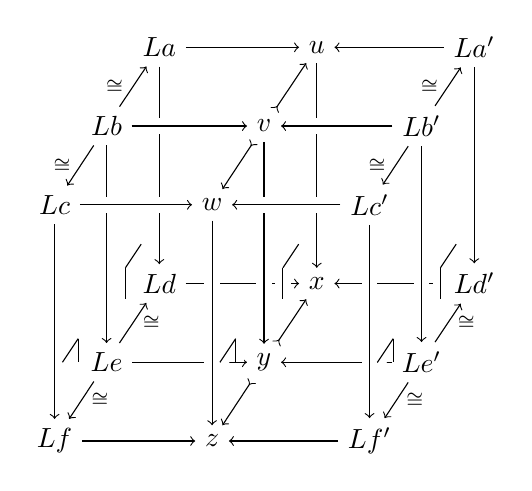
\begin{tikzpicture}
    % objects
    \node (1) at (1.33,5) {\( La \)};
    \node (2) at (3.33,5) {\( u \)};
    \node (3) at (5.33,5) {\( La' \)};
    \node (4) at (0.66,4) {\( Lb \)};
    \node (5) at (2.66,4) {\( v \)};
    \node (6) at (4.66,4) {\( Lb' \)};
    \node (7) at (0,3) {\( Lc \)};
    \node (8) at (2,3) {\( w \)};
    \node (9) at (4,3) {\( Lc' \)};
    \node (1') at (1.33,2) {\( Ld \)};
    \node (2') at (3.33,2) {\( x \)};
    \node (3') at (5.33,2) {\( Ld' \)};
    \node (4') at (0.66,1) {\( Le \)};
    \node (5') at (2.66,1) {\( y \)};
    \node (6') at (4.66,1) {\( Le' \)};
    \node (7') at (0,0) {\( Lf \)};
    \node (8') at (2,0) {\( z \)};
    \node (9') at (4,0) {\( Lf' \)};
    % back faces
    \draw [->] (1) to node [] {\scriptsize{\(  \)}} (2);
    \draw [->] (1') to node [] {\scriptsize{\(  \)}} (2');
    \draw [->] (3) to node [] {\scriptsize{\(  \)}} (2);
    \draw [->] (3') to node [] {\scriptsize{\(  \)}} (2');
    \draw [->] (1) to node [] {\scriptsize{\(  \)}} (1');
    \draw [->] (2) to node [] {\scriptsize{\(  \)}} (2');
    \draw [->] (3) to node [] {\scriptsize{\(  \)}} (3');
    % connect back to mid faces
    \draw [->] (4) to node [left] {\scriptsize{\( \iso \)}} (1);
    \draw [->] (4') to node [right] {\scriptsize{\( \iso \)}} (1');
    \draw [>->] (5) to node [] {\scriptsize{\(  \)}} (2);
    \draw [>->] (5') to node [] {\scriptsize{\(  \)}} (2');
    \draw [->] (6) to node [left] {\scriptsize{\( \iso \)}} (3);
    \draw [->] (6') to node [right] {\scriptsize{\( \iso \)}} (3');
    % mid faces white
    \draw [white, line width=2mm] (4) -- (5);
    \draw [white, line width=2mm] (4') -- (5');
    \draw [white, line width=2mm] (6) -- (5);
    \draw [white, line width=2mm] (6') -- (5');
    \draw [white, line width=2mm] (4) -- (4');
    \draw [white, line width=2mm] (5) -- (5');
    \draw [white, line width=2mm] (6) -- (6');
    % mid faces
    \draw [->] (4) to node [] {\scriptsize{\(  \)}} (5);
    \draw [->] (4') to node [] {\scriptsize{\(  \)}} (5');
    \draw [->] (6) to node [] {\scriptsize{\(  \)}} (5);
    \draw [->] (6') to node [] {\scriptsize{\(  \)}} (5');
    \draw [->] (4) to node [] {\scriptsize{\(  \)}} (4');
    \draw [->] (5) to node [] {\scriptsize{\(  \)}} (5');
    \draw [->] (6) to node [] {\scriptsize{\(  \)}} (6');
    % connect front to mid faces white
    \draw [white, line width=2mm] (4) -- (7);
    \draw [white, line width=2mm] (5) -- (8);
    \draw [white, line width=2mm] (6) -- (9);
    \draw [white, line width=2mm] (4') -- (7');
    \draw [white, line width=2mm] (5') -- (8');
    \draw [white, line width=2mm] (6') -- (9');
    % connect front to mid faces
    \draw [->] (4) to node [left] {\scriptsize{\( \iso \)}} (7);
    \draw [>->] (5) to node [] {\scriptsize{\(  \)}} (8);
    \draw [->] (6) to node [left] {\scriptsize{\( \iso \)}} (9);
    \draw [->] (4') to node [right] {\scriptsize{\( \iso \)}} (7');
    \draw [>->] (5') to node [] {\scriptsize{\(  \)}} (8');
    \draw [->] (6') to node [right] {\scriptsize{\( \iso \)}} (9');
    % front faces white
    \draw [white, line width=2mm] (7) -- (8);
    \draw [white, line width=2mm] (9) -- (8);
    \draw [white, line width=2mm] (7') -- (8');
    \draw [white, line width=2mm] (9') -- (8');
    \draw [white, line width=2mm] (7) -- (7');
    \draw [white, line width=2mm] (8) -- (8');
    \draw [white, line width=2mm] (9) -- (9');
    % front faces
    \draw [->] (7) to node [] {\scriptsize{\(  \)}} (8);
    \draw [->] (9) to node [] {\scriptsize{\(  \)}} (8);
    \draw [->] (7') to node [] {\scriptsize{\(  \)}} (8');
    \draw [->] (9') to node [] {\scriptsize{\(  \)}} (8');
    \draw [->] (7) to node [] {\scriptsize{\(  \)}} (7');
    \draw [->] (8) to node [] {\scriptsize{\(  \)}} (8');
    \draw [->] (9) to node [] {\scriptsize{\(  \)}} (9');
    % left pushouts 
    \draw (1.1,2.5) -- (0.9,2.2);
    \draw (0.9,2.2) -- (0.9,1.8);
    \draw (0.3,1.3) -- (0.1,1);
    \draw (0.3,1.3) -- (0.3,1);
    % mid pushouts white
    \draw [white, line width=2mm] (3.1,2.5) -- (2.9,2.2);
    \draw [white, line width=2mm] (2.9,2.2) -- (2.9,1.8);
    \draw [white, line width=2mm] (2.3,1.3) -- (2.1,1);
    \draw [white, line width=2mm] (2.3,1.3) -- (2.3,1);
    % mid pushouts 
    \draw (3.1,2.5) -- (2.9,2.2);
    \draw (2.9,2.2) -- (2.9,1.8);
    \draw (2.3,1.3) -- (2.1,1);
    \draw (2.3,1.3) -- (2.3,1);
    % left pushouts white
    \draw [white, line width=2mm] (5.1,2.5) -- (4.9,2.2);
    \draw [white, line width=2mm] (4.9,2.2) -- (4.9,1.8);
    \draw [white, line width=2mm] (4.3,1.3) -- (4.1,1);
    \draw [white, line width=2mm] (4.3,1.3) -- (4.3,1);
    % left pushouts 
    \draw (5.1,2.5) -- (4.9,2.2);
    \draw (4.9,2.2) -- (4.9,1.8);
    \draw (4.3,1.3) -- (4.1,1);
    \draw (4.3,1.3) -- (4.3,1);

  \end{tikzpicture}
\]
% 

Hence, given a linear production of structured cospans, Lemma
\ref{thm:po-respect-monics} ensures that any derived production is
also linear.


To build the language, after the derivation comes generating a
category, which we did in Section \ref{sec:yrewriting-strcsp} with a
functor 
%
\(
  S \from \Gram \to \Cat.
\)
% 
In this section, we define a similar functor
%
\(
  S\lin \from \Gram\lin \to \DblCat.
\)
% 
Before we show how $ S\lin $ works, we recall a few important
concepts.

\begin{lemma}

  Given a topos $ \cat{T} $, there is a symmetric monoidal double
  category $ \MMMonRewrite (\cat{T}) $ whose
  \begin{itemize}
  \item objects are the $ \cat{T} $-objects,
  \item vertical arrows are isomorphism classes of spans with
    invertible legs in $ \cat{T} $,
  \item horizontal arrows are cospans in $ T $, and
  \item squares are commuting diagrams of the form
    %
    \[
      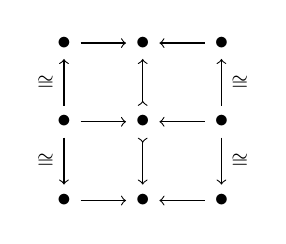
\begin{tikzpicture}
        \node (1) at (0,2) {\( \bullet \)};
        \node (2) at (1,2) {\( \bullet \)};
        \node (3) at (2,2) {\( \bullet \)};
        \node (4) at (0,1) {\( \bullet \)};
        \node (5) at (1,1) {\( \bullet \)};
        \node (6) at (2,1) {\( \bullet \)};
        \node (7) at (0,0) {\( \bullet \)};
        \node (8) at (1,0) {\( \bullet \)};
        \node (9) at (2,0) {\( \bullet \)};
        \draw [->] (1) to node [] {\scriptsize{\(  \)}} (2);
        \draw [->] (3) to node [] {\scriptsize{\(  \)}} (2);
        \draw [->] (4) to node [] {\scriptsize{\(  \)}} (5);
        \draw [->] (6) to node [] {\scriptsize{\(  \)}} (5);
        \draw [->] (7) to node [] {\scriptsize{\(  \)}} (8);
        \draw [->] (9) to node [] {\scriptsize{\(  \)}} (8);
        \draw [->] (4) to node [left] {\scriptsize{\( \iso \)}} (1);
        \draw [->] (4) to node [left] {\scriptsize{\( \iso \)}} (7);
        \draw [>->] (5) to node [] {\scriptsize{\(  \)}} (2);
        \draw [>->] (5) to node [] {\scriptsize{\(  \)}} (8);
        \draw [->] (6) to node [right] {\scriptsize{\( \iso \)}} (3);
        \draw [->] (6) to node [right] {\scriptsize{\( \iso \)}} (9);
      \end{tikzpicture}
    \]
    % 
  in $ \cat{T} $
  \end{itemize}

  The symmetric monoidal operation is defined pointwise.
  %
  \todo{cite spcsptopos}
  %

\end{lemma}

The compositions in this category follow as they do in
%
\(
  \Span{\StrCsp\ob (L)}
\)
% 
and
%
\(
  \StrCsp\arr (L).
\)

Note that a linear production taken from a structured cospan category
$ \StrCsp\ob (L) $ with invertible maps for legs has the correct form to
be a square in
%
\(
  \MMMonRewrite ( \X )
\)
% 
where $ \X $ is the domain of $ L $.  Thus a linear grammar
$ ( \StrCsp\ob (L) , P ) $ generates a sub-double category $ \PPP $ of
%
\(
  \MMMonRewrite ( \X ).
\)
%
In fact, we can do so functorially.

\begin{theorem} \label{thm:s-lin-functor}

  There is a functor $ S\lin \from \Gram\lin \to \DblCat $ given by
  \begin{itemize}
  \item $ ( \StrCsp\ob (L) , P ) \mapsto \PPP $,
  \item
    %
    \(
      F \from
      ( \StrCsp\ob (L) , P ) \to ( \StrCsp\ob (L') , P' ) 
    \)
    % 
    is sent to the double functor $ \PPP \to \PPP' $ defined on
    squares by
    %
    % \[
    %   \begin{tikzpicture}
    %     \node (1) at () {\(  \)};
    %     \node (2) at () {\(  \)};
    %     \node (3) at () {\(  \)};
    %     \node (4) at () {\(  \)};
    %     \node (5) at () {\(  \)};
    %     \node (6) at () {\(  \)};
    %     \node (7) at () {\(  \)};
    %     \node (8) at () {\(  \)};
    %     \draw [->] () to node [] {\scriptsize{\(  \)}} ();
    %     \draw [->] () to node [] {\scriptsize{\(  \)}} ();
    %     \draw [->] () to node [] {\scriptsize{\(  \)}} ();
    %     \draw [->] () to node [] {\scriptsize{\(  \)}} ();
    %     \draw [->] () to node [] {\scriptsize{\(  \)}} ();
    %     \draw [->] () to node [] {\scriptsize{\(  \)}} ();
    %     \draw [->] () to node [] {\scriptsize{\(  \)}} ();
    %     \draw [->] () to node [] {\scriptsize{\(  \)}} (); 
    %   \end{tikzpicture}
    % \]
    % % 


    %
    \[
      \begin{tikzpicture}
        \begin{scope}
        \node (1) at (0,4) {\( La  \)};
        \node (2) at (2,4) {\( x \)};
        \node (3) at (4,4) {\( La' \)};
        \node (4) at (0,2) {\( Lb \)};
        \node (5) at (2,2) {\( y \)};
        \node (6) at (4,2) {\( Lb' \)};
        \node (7) at (0,0) {\( Lc \)};
        \node (8) at (2,0) {\( z \)};
        \node (9) at (4,0) {\( Lc' \)};
        \draw [->] (1) to node [] {\scriptsize{\(  \)}} (2);
        \draw [->] (3) to node [] {\scriptsize{\(  \)}} (2);
        \draw [->] (4) to node [] {\scriptsize{\(  \)}} (5);
        \draw [->] (6) to node [] {\scriptsize{\(  \)}} (5);
        \draw [->] (7) to node [] {\scriptsize{\(  \)}} (8);
        \draw [->] (9) to node [] {\scriptsize{\(  \)}} (8);
        \draw [->] (4) to node [] {\scriptsize{\(  \)}} (1);
        \draw [->] (4) to node [] {\scriptsize{\(  \)}} (7);
        \draw [->] (5) to node [] {\scriptsize{\(  \)}} (2);
        \draw [->] (5) to node [] {\scriptsize{\(  \)}} (8);
        \draw [->] (6) to node [] {\scriptsize{\(  \)}} (3);
        \draw [->] (6) to node [] {\scriptsize{\(  \)}} (9);
        \end{scope}
      \end{tikzpicture}
    \]
    % 

  \end{itemize}
  
\end{theorem}

\begin{lemma} \label{thm:horbicat-MMonRewrite}

  The horizontal bicategry $ \MMonRewrite ( \cat{T} ) $ of
  $ \MMMonRewrite ( \cat{T} ) $ is compact closed.
  %
  \todo{cite spcsptopos}
  %
  
\end{lemma}

% ~~~~~~~~~~~~~~~~~~~~~~~~~~~~~~~~~~~~
% ~~~~~~~~~~~~~~~~~~~~~~~~~~~~~~~~~~~~
% ~~~~~~~~~~~~~~~~~~~~~~~~~~~~~~~~~~~~
% ~~~~~~~~~~~~~~~~~~~~~~~~~~~~~~~~~~~~

\section{Languages for left-linear grammars}
\label{sec:lang-left-linear-grammars}












% Finding the derived grammar is only one step in the generative
% process we are outlining. The next is to use a derived grammar to
% functorially construct a bicategory. However, before commencing
% construction on this bicategory, we begin our slow transition to our
% ultimate destination, rewriting structured cospans. In particular, we
% show that structured cospans are compatible with DPO rewriting.

% \begin{definition} % contstruct a bicat from a derived grammar

%   Let $ DG $ be derived from the grammar $ G \coloneqq ( \C , P )
%   $. Define a bicategory with
%   \begin{itemize}
%   \item $ \C $-objects as objects,
%   \item cospans in $ \C $ as arrows,
%   \item spans of cospans
%     %
%     \[
%       \begin{tikzpicture}
%         \node (1) at () {\( a \)};
%         \node (2) at () {\( \ell \)};
%         \node (3) at () {\( k \)};
%         \node (4) at () {\( r \)};
%         \node (5) at () {\( b \)};
%         \draw [->] (1) to node [] {\scriptsize{\(  \)}} (2);
%         \draw [->] (1) to node [] {\scriptsize{\(  \)}} (3);
%         \draw [->] (1) to node [] {\scriptsize{\(  \)}} (4);
%         \draw [->] (5) to node [] {\scriptsize{\(  \)}} (2);
%         \draw [->] (5) to node [] {\scriptsize{\(  \)}} (3);
%         \draw [->] (5) to node [] {\scriptsize{\(  \)}} (4);
%         \draw [>->] (3) to node [] {\scriptsize{\(  \)}} (2);
%         \draw [>->] (3) to node [] {\scriptsize{\(  \)}} (4); 
%       \end{tikzpicture}
%     \]
%     %
%     for any production $ \ell \gets k \to r $ as 2-arrows.     
%   \end{itemize}

%   \edit{there's also the bicateogyr of relations case too}

%   \edit{ maybe I should straight up define this using a
%     geom. morphism, and 0-cells are A, 1-cells are structured cospans,
%     and 2-cells are generated by spans of cospans l <-- k --> r with La
%     and Lb going into each l,k,r, for all productions derived from a
%     set of productions.  }
%   \end{definition}
%   

% \end{definition}






% ~~~~~~~~~~~~~~~~~~~~~~~~~~~~~~~~~~~~
% ~~~~~~~~~~~~~~~~~~~~~~~~~~~~~~~~~~~~


% \subsection{A bicategory for rewriting}
% \label{sec:bicat-rewriting}



% \begin{definition}

%   There is a double category $ \RRRewrite $ consisting of
%   %
%   \begin{itemize}
%   \item $ \A $-objects for objects,
%   \item cospans in $ \A $ with invertible legs for vertical arrows,
%   \item structured cospans $ La \to x \gets Lb $ as horizontal arrows
%     of type $ a \nrightarrow b $, and
%   \item commuting diagrams
%     %
%     \[
%       \begin{tikzpicture}
%         \node (1) at (-1,1) {\( La \)};
%         \node (2) at (0,1) {\( x \)};
%         \node (3) at (1,1) {\( La' \)};
%         \node (4) at (-1,0) {\( Lb \)};
%         \node (5) at (0,0) {\( y \)};
%         \node (6) at (1,0) {\( Lb' \)};
%         \node (7) at (-1,-1) {\( Lc \)};
%         \node (8) at (0,-1) {\( z \)};
%         \node (9) at (1,-1) {\( Lc' \)};
%         \draw [->] (1) to node [] {\scriptsize{\(  \)}} (2);
%         \draw [->] (3) to node [] {\scriptsize{\(  \)}} (2);
%         \draw [->] (4) to node [] {\scriptsize{\(  \)}} (5);
%         \draw [->] (6) to node [] {\scriptsize{\(  \)}} (5);
%         \draw [->] (7) to node [] {\scriptsize{\(  \)}} (8);
%         \draw [->] (9) to node [] {\scriptsize{\(  \)}} (8);
%         \draw [->] (4) to node [] {\scriptsize{\( \cong \)}} (1);
%         \draw [->] (4) to node [] {\scriptsize{\( \cong \)}} (7);
%         \draw [->] (5) to node [] {\scriptsize{\( \cong \)}} (2);
%         \draw [->] (5) to node [] {\scriptsize{\( \cong \)}} (8);
%         \draw [->] (6) to node [] {\scriptsize{\( \cong \)}} (3);
%         \draw [->] (6) to node [] {\scriptsize{\( \cong \)}} (9); 
%       \end{tikzpicture}
%     \]
%     % 
%     as 2-arrows.
%   \end {itemize}
%   %
% \end{definition}

% \begin{definition}

%   There is a bicategory $ \RRewrite $ consisting of
%   %
%   \begin{itemize}
%   \item $ \A $-objects for objects
%   \item structured cospans $ La \to x \gets Lb $ as arrows of type $ a
%     \to b $, and
%   \item commuting diagrams
%     %
%     \[
%       \begin{tikzpicture}
%         \node (1) at (-1,0) {\( La \)};
%         \node (2) at (0,1) {\( x \)};
%         \node (3) at (0,0) {\( y \)};
%         \node (4) at (0,-1) {\(z \)};
%         \node (5) at (1,0) {\( Lb \)};
%         \draw [->] (1) to node [] {\scriptsize{\(  \)}} (2);
%         \draw [->] (5) to node [] {\scriptsize{\(  \)}} (2);
%         \draw [->] (1) to node [] {\scriptsize{\(  \)}} (3);
%         \draw [->] (5) to node [] {\scriptsize{\(  \)}} (3);
%         \draw [->] (1) to node [] {\scriptsize{\(  \)}} (4);
%         \draw [->] (5) to node [] {\scriptsize{\(  \)}} (4);
%         \draw [>->] (3) to node [] {\scriptsize{\(  \)}} (2);
%         \draw [>->] (3) to node [] {\scriptsize{\(  \)}} (4); 
%       \end{tikzpicture}
%     \]
%     % 
%     as 2-arrows.
%   \end{itemize}
%   %
% \end{definition}



% % ~~~~~~~~~~~~~~~~~~~~~~~~~~~~~~~~~~~~~~~~
% % ~~~~~~~~~~~~~~~~~~~~~~~~~~~~~~~~~~~~~~~~
% % ~~~~~~~~~~~~~~~~~~~~~~~~~~~~~~~~~~~~~~~~
% % ~~~~~~~~~~~~~~~~~~~~~~~~~~~~~~~~~~~~~~~~

% \section{Examples}
% \label{sec:examples}

% % ~~~~~~~~~~~~~~~~~~~~~~~~~~~~~~~~~~~~~~~~
% % ~~~~~~~~~~~~~~~~~~~~~~~~~~~~~~~~~~~~~~~~
% % ~~~~~~~~~~~~~~~~~~~~~~~~~~~~~~~~~~~~~~~~
% % ~~~~~~~~~~~~~~~~~~~~~~~~~~~~~~~~~~~~~~~~

% %\bibliography{C:/Dropbox/templates/biblio.bib} 
% %\bibliographystyle{ieeetr}

% %\begin{thebibliography}{99}
% %\end{thebibliography}

% ~~~~~~~~~~~~~~~~~~~~~~~~~~~~~~~~~~~~~~~~
% 
% ~~~~~~~~~~~ end document ~~~~~~~~~~~~~~~
% 
% ~~~~~~~~~~~~~~~~~~~~~~~~~~~~~~~~~~~~~~~~

\end{document}
